\chapter{Discussion and Future Perspectives}
\label{ch:limitations_perspectives}

\section{Limitations and future perspectives}
\label{sec:limitations_perspectives}

The contributions presented in Chapters \ref{ch:gvamp} and \ref{ch:vampw}---focusing on joint inference in large-scale \gls{gwas} and the impact of proteomics on disease onset--- establish a foundation for further research. While the application of \acrlong{vamp} algorithms to high-dimensional biological data offers significant advantages, several underlying limitations remain. In this section, we outline these constraints in the context of omics data and complex traits, as well as potential avenues for future research.

% While \gls{vamp} is designed to handle ill-conditioned matrices, its theoretical guarantees assume uniform right singular vectors---an assumption often violated by the highly correlated data setups of interest in fine-mapping. Because of the resulting convergence issues, its application is currently restricted to scenarios mixing common and numerous rare variants, excluding the dense, extremely correlated loci that are of ultimate biological interest. A second major limitation involves hyperparameter learning. Although our approaches demonstrate improved variable selection and prediction accuracy, they can struggle to learn stable hyperparameters, instead oscillating between multiple fixed points. As a result, this limits biological interpretability and the conclusions drawn about these quantities. To address the intrinsic convergence issues, one promising direction involves reframing the estimation problem within a constrained optimization framework \cite{Slock2022}.

% From a computational standpoint, the gVAMP algorithm is memory-bound, explicitly trading RAM for execution speed by loading the entire PLINK genotype matrix into memory. To alleviate this constraint, future iterations could implement an out-of-core streaming approach, reading the genotype data in discrete chunks to restrict peak memory usage to just a few gigabytes. Similar streaming techniques have already been integrated into other genomic frameworks to manage high-dimensional data \cite{hof2024ldak}.

While \gls{vamp} is designed to handle ill-conditioned matrices, its theoretical guarantees assume uniform right singular vectors---an assumption often violated by the highly correlated data setups of interest in fine-mapping analyses. Because of the resulting convergence issues, its application in genomics is currently restricted to scenarios mixing common and numerous rare variants, excluding the dense, extremely correlated loci that are of ultimate biological interest. A second major limitation involves hyperparameter learning. Although our approaches demonstrate improved variable selection and prediction accuracy, they can struggle to learn stable hyperparameters, instead oscillating between multiple fixed points. As a result, this limits biological interpretability and the conclusions drawn about these quantities. Furthermore, from a computational standpoint, the gVAMP algorithm is inherently memory-bound, explicitly trading RAM for execution speed by loading the entire PLINK genotype matrix into memory.

To address these theoretical and computational challenges, several promising directions exist for future iterations. The intrinsic convergence issues could potentially be mitigated by reframing the estimation problem within a constrained optimization framework \cite{Slock2022}. Concurrently, to alleviate the strict memory constraints, the algorithm could implement an out-of-core streaming approach. By reading the genotype data in discrete chunks, peak memory usage could be restricted to just a few gigabytes---a technique already integrated into other genomic frameworks to manage high-dimensional data \cite{hof2024ldak}.

% These theoretical limitations do not undermine the practical utility of Approximate Message Passing approaches in computational omics. Specifically, recent universality results for right-rotationally invariant models \cite{dudeja2022universality,Wang22AMPUniversality} suggest that the theoretical underpinnings of these algorithms can remain correct even under departures from original assumptions. Furthermore, the successful application of this framework across the preceding chapters highlights its value for large-scale biological analysis. Also, one promising direction involves reframing the estimation problem within a constrained optimization framework \cite{Slock2022}. 

% Nonetheless, resolving the divergence issues intrinsic to AMP remains a primary concern for future applications. One promising direction involves reframing the estimation problem within a constrained optimization framework \cite{Slock2022}. 

\subsection{Alternative approximate message passing frameworks}

Future reductions in algorithmic complexity compared to the VAMP-based approach could be achieved by adopting the Memory Approximate Message Passing (MAMP) framework \cite{MAMP}. MAMP effectively lowers the computational burden to match that of standard \gls{amp} by incorporating estimators from previous iterations when constructing a noisy signal estimate. A closely related approach is Orthogonal Message Passing (OAMP) \cite{OAMP}, which shares a similar algorithmic structure with VAMP; in fact, the two methods are equivalent when OAMP is implemented with a specific variance updating rule.

Building on these foundations, recent theoretical work has introduced Generalized OAMP (GOAMP) tailored specifically for sublinear sparsity \cite{takeuchi2025generalized}. This framework addresses regimes where the number of non-zero effect sizes grows sublinearly with respect to the total number of variants, i.e., assuming that $\lim_{P, \text{CV} \to \infty} \log \text{CV} / \log P = \gamma \in [0, 1)$, where $\text{CV}$ represents the number of causal variants and $P$ is the total number of variants. Compared to the standard OAMP, this approach alters the asymptotic variance estimation. Hence, adapting such a sublinear inference procedure in statistical genetics holds promise for improving variable selection in highly sparse, oligogenic traits. Blood biomarkers provide a clear use case for such a procedure; for instance, the genetic architecture of Lipoprotein(a) is exceptionally sparse, with variation localized almost entirely within the $LPA$ gene region on chromosome 6 accounting for over 90\% of plasma concentration variance \cite{Boerwinkle,Clarke}. A similar pattern is observed in total bilirubin levels, where the top 1\% of loci explain 60.9\% of the \gls{snp} heritability \cite{35blood_biomarkers}. Applying GOAMP-based estimators to these phenotypes could yield more accurate \acrlongpl{pip} for the small subset of causal loci underlying these biomarker levels.

\subsection{Transfer learning for multi-ancestry prediction}

We also suggest extending the inference framework to models that account for the heterogeneity of the population, specifically setups in which the population is composed of individuals of different genetic ancestry. To explore transfer learning abilities from an overrepresented subpopulation to underrepresented subpopulations, several \gls{mcmc} approaches have been developed. These methods that either directly model the correlation between ancestry-specific effect sizes via global hyperparameters \cite{prscsx,mussel,JointPRS} or use the posterior mean of the overrepresented population in the prior construction for underrepresented subpopulations \cite{BridgePRS}. Upon estimating the effect sizes for all subpopulations, a typical approach is to fit a simple linear regression model between the predictors obtained from each subpopulation and tune hyperparameters on the validation set of the targeted subpopulation. 

Hence, motivated by the approach taken by \cite{BridgePRS} and work on AMP with side information \cite{AMP_side_info}, we propose conditioning on an additional state evolution result from the overrepresented population when constructing denoisers for the underrepresented population. A predictor obtained in this way would represent a transfer learning component from one subpopulation to the other, implicitly searching for shared effect sizes, while performing training only on the targeted subpopulation. Such an approach would retain the advantages of individual-level models over summary-level models while remaining highly computationally efficient. This efficiency is achieved because the effect sizes and state evolution parameters for the overrepresented population only need to be computed once, and training individual-level models for underrepresented subpopulations is much faster due to their smaller sample sizes.
% Such an approach would enjoy the benefits derived from using individual-level models over summary-level models, while being extremely computationally efficient, as the overrepresented population effect sizes and state evolution parameters would need to be calculated only once, and since training individual-level models in underrepresented subpopulations is much faster due to a lower number of individuals involved. 
In terms of objects from Algorithm \ref{gVAMP}, instead of deriving 
\begin{equation}
    \mathbb{E}[\bm{\beta}|{{\bm{r}_{1,t}}^{(2)}} = \mathcal{N}(\bm{\beta}, (\gamma_{1,t}^{(2)})^{-1} \bm{I}), \Theta_{t}]
\end{equation}
for the underrepresented population, we propose deriving 
\begin{equation}
    \mathbb{E}[\bm{\beta} | {\bm{r}_{1,t}}^{(2)} = \mathcal{N}(\bm{\beta}, ({\gamma_{1,t}}^{(2)})^{-1} \bm{I}), {{\bm{r}_1}^{(1)}} = \mathcal{N}(\bm{\beta}, ({\gamma_{1}}^{(1)})^{-1} \bm{I}), \Theta_{t}],
\end{equation}
where the objects ${\bm{r}_{1,t}}^{(2)} \text{ and } {\gamma_{1,t}}^{(2)}$ relate to the underrepresented population and the objects ${{\bm{r}_1}^{(1)}} \text{ and } {\gamma_{1}}^{(1)}$ represent VAMP objects and state evolution parameters taken from the stopping iteration of the training on the overrepresented subpopulation. The detailed derivation of these denoisers is provided in Supplementary Section \ref{supp:note3}. Our preliminary analysis suggests that the proposed transfer learning approach modestly outperforms the widely used multi-ancestry inference method PRScsx \cite{prscsx} for standing height and body mass index, specifically when transferring information from the European to the South Asian subpopulation in the UK Biobank, as defined by self-reported ancestry.

\subsection{Beyond standard linear models}

Moving beyond standard Bayesian linear models, future work could also extend these frameworks to accommodate diverse outcome distributions. This includes modeling binary phenotypes via Bayesian logistic or probit regression, as well as handling count data through a Poisson model, following the theoretical framework established in \cite{schniter_vector_2016}.

% Alternatively, these message-passing techniques can be generalized to more complex non-linear architectures; for instance, the Multi-Layer VAMP framework \cite{MultiLayerVAMP} enables inference across deep neural networks while maintaining a rigorous state evolution result that tracks the distributions of iterates. Such an approach could provide a powerful tool for modeling and inferring the epistatic effects that the genome or proteome exerts on a complex trait.

As an extension of these approaches, future work could improve predictive performance by incorporating functional annotations through grouped priors \cite{bayesrc} or by transitioning to joint inference across multiple correlated traits to increase statistical power.

\subsection{Extending gVAMP to summary statistics}

While the methods presented in this thesis demonstrate strong performance on the individual level data, the primary obstacle to broader applicability of these approaches remains the restricted availability of raw genotype data. Due to strict privacy regulations, genotype and phenotype records cannot be easily shared across institutions, and the direct merging of individual-level datasets from different biobanks is prohibited. Consequently, to achieve the sample sizes necessary for fully resolving complex traits, the field increasingly relies on summary statistics---namely, marginal effect estimates and reference \gls{ld} panels. Adapting the proposed VAMP-based algorithms to operate on these summary-level inputs represents a promising next step. This transition is feasible, as the core VAMP iterations can be mathematically reformulated to bypass individual-level information. Specifically, in the standard VAMP algorithm, the Linear Minimum Mean Squared Error (LMMSE) step requires solving the following linear system for $\hat{\bm{\beta}}_2$:

\begin{equation}
(\gamma_w \bm{X}^\top \bm{X} + \gamma_2 \bm{I}) \hat{\bm{\beta}}_2 = \gamma_w \bm{X}^\top \bm{y} + \gamma_2 \bm{r}_2,
\end{equation}

where $\bm{X}$ is the column-normalized genotype matrix, $\gamma_w$ is the noise precision, and $\bm{r}_2$ and $\gamma_2$ are passed from the preceding denoising step, with $\bm{r}_2$ asymptotically behaving as the true signal corrupted by independent Gaussian noise, and $\gamma_2$ representing the precision of that noise. By substituting the in-sample LD matrix $\bm{R} = \frac{1}{N} \bm{X}^\top \bm{X}$ and the marginal GWAS associations $\hat{\bm{\beta}}_{\text{GWAS}} = \frac{1}{N} \bm{X}^\top \bm{y}$, we can scale the entire system by the sample size $N$ to yield a purely summary-based update:

\begin{equation} 
    \bigg (\gamma_w \bm{R} + \frac{\gamma_2}{N} \bm{I} \bigg ) \hat{\bm{\beta}}_2 = \gamma_w \hat{\bm{\beta}}_{\text{GWAS}} + \frac{\gamma_2}{N} \bm{r}_2.
\end{equation}

This formulation preserves exact mathematical equivalence to the individual-level model while relying exclusively on summary statistics, thereby better protecting participant privacy. In practice, however, computing and storing the fully dense matrix $\bm{R}$ is computationally prohibitive for large-scale data. Consequently, $\bm{R}$ is typically replaced by an estimator $\hat{\bm{R}}$---such as a banded, block-diagonal, or sparse-thresholded approximation, as discussed in Section \ref{subsec:summary_level_prs}. Furthermore, similar to the theoretical approach proposed for transfer learning, one could develop a VAMP-based algorithm for joint inference across $K$ summary-statistic sources. Assuming that these sources share the same underlying Bayesian linear model and corresponding effect size vector $\bm{\beta}$, the LMMSE steps could be executed separately for each source. The shared knowledge would then be integrated during the denoising step. Instead of utilizing the standard single-source denoiser 
\begin{equation}
    \mathbb{E}[\bm{\beta} \mid \bm{r}_{1,t} = \bm{\beta} + \mathcal{N}(0, \gamma_{1,t}^{-1}\bm{I}), \Theta_{t}],
\end{equation} 
the framework would employ a multi-source denoiser conditioned on the noisy signal measurements and precisions from all $K$ datasets:
\begin{equation}
    \mathbb{E}[\bm{\beta} \mid \bm{r}_{1,t}^{(1)} = \bm{\beta} + \mathcal{N}(0, (\gamma_{1,t}^{(1)})^{-1}\bm{I}), \dots, \bm{r}_{1,t}^{(K)} = \bm{\beta} + \mathcal{N}(0, (\gamma_{1,t}^{(K)})^{-1}\bm{I}), \Theta_{t}]
\end{equation}

Here, $\Theta_{t}$ represents the prior distribution hyperparameters. The variables $\bm{r}_{1,t}^{(i)}$ and $\gamma_{1,t}^{(i)}$ are derived by running the baseline summary-statistics gVAMP algorithm's LMMSE step on the $i$-th source, with $\bm{r}_{1,t}^{(i)}$ asymptotically behaving as a noisy measurement of the signal, and $\gamma_{1,t}^{(i)}$ representing the precision of that noise. The \acrlong{em} updates for the prior probabilities and noise precision can be derived following analogous principles to those used in gVAMP.

\begin{figure}[htbp]
    \centering
    \captionsetup[subfigure]{position=top, justification=raggedright, singlelinecheck=false}
    \begin{subfigure}{0.45\textwidth}
        \caption{}
        \centering
        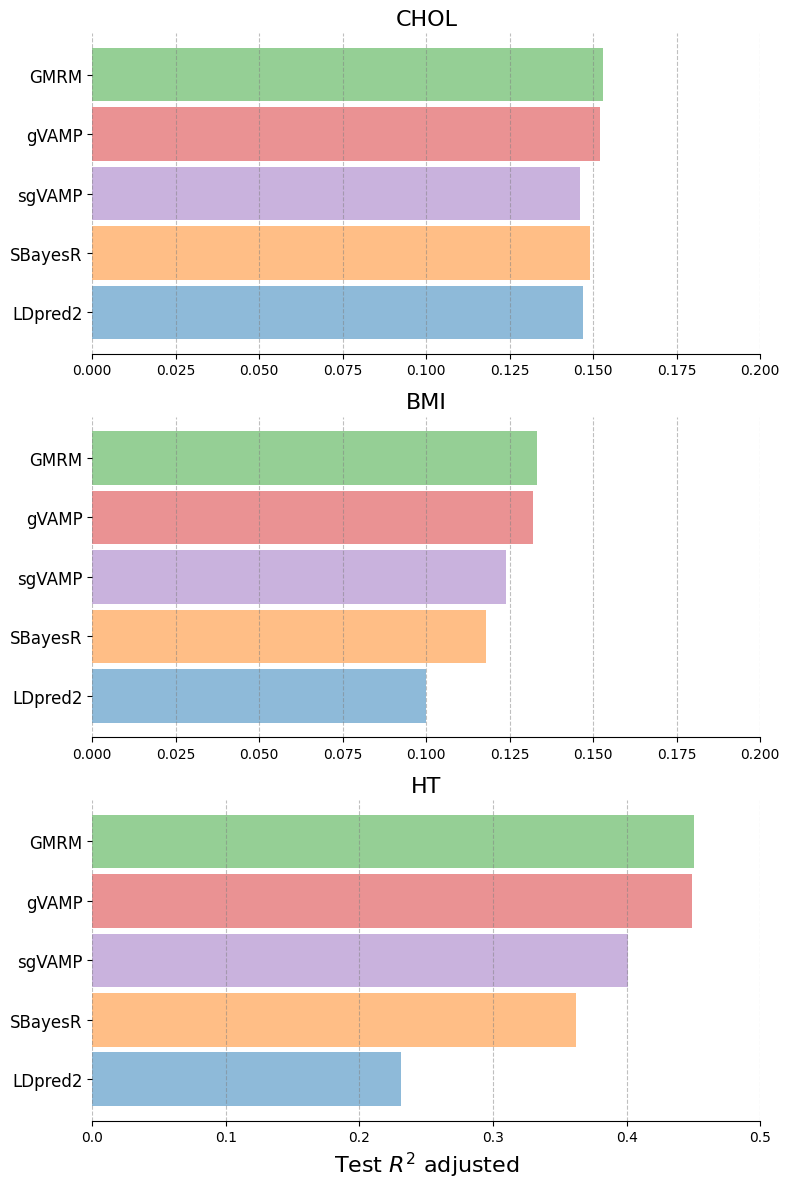
\includegraphics[width=\textwidth]{graphics/conclusion_figures/sgvamp_benchmarks.png}
        \label{fig:sgvamp_sub1}
    \end{subfigure}%
    \hfill
    \begin{subfigure}{0.45\textwidth}
        \caption{}
        \centering
        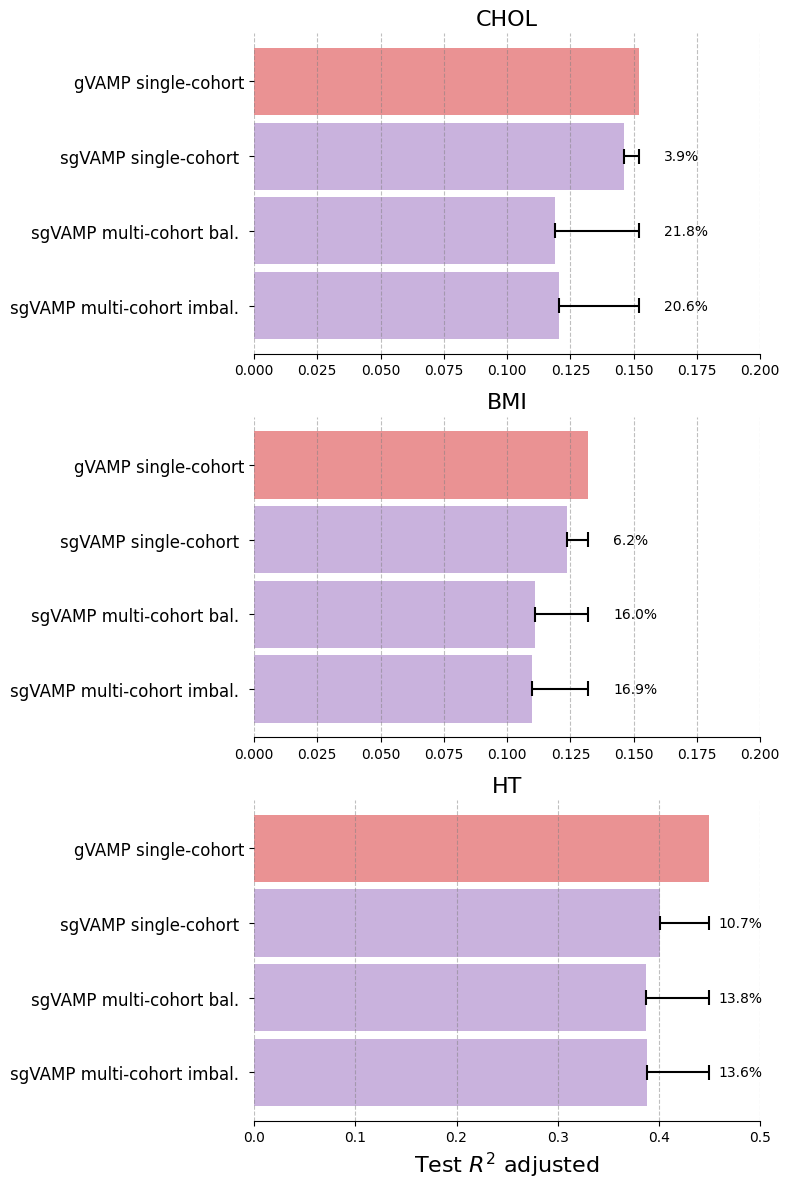
\includegraphics[width=\textwidth]{graphics/conclusion_figures/sgvamp_ukb_splits.png}
        \label{fig:sgvamp_sub2}
    \end{subfigure}
  
    \caption[Out-of-sample predictive performance of sgVAMP compared to established PRS methods and across multi-cohort splits]{\textbf{Out-of-sample predictive performance of sgVAMP compared to established PRS methods and across multi-cohort splits.} \textbf{(a)} Out-of-sample performance benchmark of sgVAMP against widely adopted polygenic risk score methods across three traits: Cholesterol (CHOL), Body Mass Index (BMI), and Standing Height (HT). The horizontal bar plots compare predictive performance (adjusted test $R^2$) across GMRM \cite{bayesrc} (green), gVAMP \cite{Depope2026} (red), sgVAMP (purple), SBayesR \cite{sbayesr} (orange), and LDpred2 \cite{ldpred} (blue). sgVAMP, the summary-level variant of gVAMP, maintains a high level of predictive accuracy, performing slightly below the individual-level state-of-the-art methods (GMRM, gVAMP) while significantly outperforming other summary-level methods for BMI and HT. The sgVAMP analysis was performed per chromosome using banded LD matrix approximations with a 1,000 kb window. Results for other methods are adapted from \cite{Depope2026}. \textbf{(b)} Predictive performance of sgVAMP in a split-cohort experiment on the UK Biobank data for CHOL, BMI, and HT. The training set was divided into either two equally sized groups (multi-cohort bal.) or two groups with a 3:1 ratio (multi-cohort imbal.). While there is an expected performance gap compared to the individual-level model trained on the full cohort, predictive accuracy remains consistent between the balanced and imbalanced data splits.}
    \label{fig:sgvamp}
\end{figure}
Figure \ref{fig:sgvamp}(a) compares the adjusted test $R^2$ performance of individual-level methods (GMRM \cite{bayesrc} and gVAMP \cite{Depope2026}) against summary-statistics methods, including our proposed summary-level version of gVAMP (sgVAMP), SBayesR \cite{sbayesr}, and LDpred2 \cite{ldpred}. Figure \ref{fig:sgvamp}(b) presents the results of a split-cohort experiment conducted on the UK Biobank dataset. We divided the training set into either two equally sized groups ("multi-cohort bal.") or two groups with a 3:1 size ratio ("multi-cohort imbal."). We evaluated the predictive performance for Cholesterol (CHOL), Body Mass Index (BMI), and Standing Height (HT) across these splits and compared it to the individual-level model trained on the full cohort. As anticipated, there is a performance gap between multi-cohort sgVAMP and the sgVAMP or gVAMP models trained on the complete dataset. Interestingly, the balanced and imbalanced split scenarios yield roughly similar predictive accuracy.

\subsection{vampW for proteomic discovery at scale}

Finally, a compelling path for future research is to apply the vampW methodology introduced in Chapter \ref{ch:vampw} to the full \gls{ukb_ppp} resource once the 600,000-sample expansion is finalized in 2027. Integrating a high-plex panel of 5,400 proteins at this scale will likely uncover substantial biological signal that remains statistically underpowered in the existing dataset. By utilizing the vampW framework, these future analyses can achieve a significant boost in discovery power while maintaining the rigorous \acrlong{fdr} control that traditional time-to-event variable selection approaches often lack.

Taking a long-term perspective, the scalability of VAMP-based inference makes it a promising candidate for the complex task of multi-omic data fusion. Integrating genomic, epigenetic, and proteomic data within a unified message-passing framework would facilitate a more holistic understanding of the regulatory networks and latent causal pathways that drive complex phenotypic traits.


\section{Conclusion}

This thesis presents novel high-dimensional statistical algorithms, built upon the Vector Approximate Message Passing framework, for joint modeling in large-scale genomics and in time-to-event proteomics data. By adopting a new perspective on inference, we move beyond the standard MCMC and variational inference techniques that form the basis of most current genome-wide association studies. A central contribution of this work is not just in the theoretical derivation of these algorithms, but in proving their practical feasibility and usefulness in large-scale computational omics. In doing so, this research bridges the gap between abstract algorithm design, scalable software implementation, and biological insights at the biobank scale.

Chapter 2 introduces gVAMP, a novel Bayesian whole-genome regression approach capable of fitting tens of millions of whole-genome sequence variants jointly for hundreds of thousands of individuals. We scale up the standard VAMP framework and combine techniques to mitigate the divergence issues commonly associated with Approximate Message Passing algorithms applied to correlated setups. Consequently, gVAMP enables joint inference at a biobank scale that far exceeds the limits of previous state-of-the-art approaches for individual-level genetic data \cite{regenie,Orliac2022}. 

By controlling for local and long-range linkage disequilibrium, it offers well-calibrated posterior inclusion probabilities that exhibit a significantly lower false discovery rate than current state-of-the-art fine-mapping methods \cite{susie,10.1093/bioinformatics/btw018}. Its capacity to handle massive whole-genome sequence inputs while providing reliable variable selection represents an important step towards a more accurate characterization of the genetic architecture of human traits. For instance, the application of gVAMP to human height data in the UK Biobank has yielded novel insights into the significant contribution of rare variation, potentially offering new avenues for prioritizing relevant genomic regions, genes, and therapeutic targets. Finally, gVAMP serves as a highly accurate tool for polygenic risk score prediction, achieving the highest reported prediction accuracy for standing human height to date. 

Chapter 3 introduces vampW, a fully parametric Bayesian survival model based on the VAMP framework for the analysis of time-to-event outcomes. We demonstrate that vampW can be applied to highly correlated proteomics data, allowing for increased prediction accuracy through the joint modeling of thousands of plasma proteins. In contrast to commonly used marginal testing and other forms of joint \acrlong{coxph}, vampW substantially reduces the false discovery rate at a similar true positive rate. The application of vampW to 24 disease outcomes in the UK Biobank study identified 219 robust protein-disease associations, many of which were missed by marginal testing. Furthermore, vampW achieves a significant improvement in the out-of-sample prediction of absolute disease onset times compared to both traditional and deep learning methods \cite{tibshirani_lasso_1997,katzman_deepsurv_2018}. These and similar future investigations have the potential to lead to a better understanding of the proteomic factors that influence when disease symptoms first appear, thereby paving the way toward personalized preventative medicine.